\section*{Experiment 1: Probabilistic Reasoning (Conjunction Fallacy)}

\subsection*{1.1. Experimental Setup and Protocol}
\textbf{Objective:} To measure the "Representativeness Heuristic" and identify whether narrative plausibility overrides the extensional rule of probability ($P(A \cap B) \leq P(A)$).

\textbf{Contamination Control:} 
To avoid data contamination (leakage of the classic "Linda Problem" from training sets), we constructed an original dataset of \textbf{130 biographical vignettes}. Each vignette uses a fixed demographic template with placeholders for \texttt{\{NAME\}}, \texttt{\{RACE\}}, and \texttt{\{AGE\}}, ensuring the specific combinations are unseen during training.

\textbf{Experimental Design:}
For each vignette, we generated two conditions:
\begin{itemize}
    \item \textbf{Correlated (Trap):} Comparing a profession $T$ (e.g., "bank teller") with a conjunction $T \land F_{corr}$, where $F_{corr}$ is a hobby narratively consistent with the persona (e.g., "social justice activist").
    \item \textbf{Uncorrelated (Control):} Comparing $T$ with $T \land F_{uncorr}$, where $F_{uncorr}$ is semantically neutral (e.g., "tennis player").
\end{itemize}

\textbf{Demographic Substitution:}
We used a factorial grid of 8 names (stratified by race: White, Black, Hispanic, Asian) and 3 age groups (24, 38, 55). Initial testing showed that age and gender had negligible effects ($\Delta Bias < 0.005$), so the final large-scale run focused on racial groups (520 trials per model).

\subsection*{1.2. Quantitative Results and Statistical Inference}
We utilized the \textbf{McNemar Test} for paired binary observations and introduced \textbf{Delta Bias} ($\Delta B$) --- a continuous metric measuring the shift in model confidence between conditions.

\begin{table}[h!]
\centering
\caption{Conjunction Fallacy Results: Binary errors and Effect Sizes}
\label{tab:linda_full_data}
\begin{tabular}{lccccc}
\toprule
\textbf{Model} & \textbf{$n_{21}$ (Errors in Trap)} & \textbf{McNemar $p$} & \textbf{$\Delta$ Bias} & \textbf{Cohen's $d$} & \textbf{Effect} \\ 
\midrule
qwen3-next-80b     & 316 / 520 & $1.5 \cdot 10^{-95}$ & +0.5648 & 1.456 & Very Large \\
gemma-3-27b-it     & 305 / 520 & $3.1 \cdot 10^{-92}$ & +0.4975 & 1.330 & Very Large \\
gpt-5.2            & 209 / 520 & $2.4 \cdot 10^{-63}$ & +0.3746 & 1.160 & Very Large \\
grok-4.1-fast      & 119 / 520 & $3.0 \cdot 10^{-36}$ & +0.2485 & 0.671 & Moderate-Large \\
deepseek-v3.2      & 97 / 520  & $1.3 \cdot 10^{-29}$ & +0.1996 & 0.930 & Large \\
gemma-3-12b-it     & 15 / 520  & $6.1 \cdot 10^{-5}$  & +0.0389 & 0.257 & Small-Moderate \\
glm-4.7-flash      & 26 / 3120 & $3.0 \cdot 10^{-8}$  & +0.0279 & 0.278 & Small-Moderate \\
claude-sonnet-4.6  & 1 / 520   & $1.0$                & +0.1049 & 1.619 & Very Large* \\
qwen3.5-397b       & 5 / 3120  & $0.0625$             & -0.0052 & -0.112 & Negligible \\
\bottomrule
\end{tabular}
\end{table}

\subsection*{1.3. Analysis of Model Confidence and Calibration}
A critical finding is that models are not merely "guessing"; they exhibit high subjective certainty in their incorrect answers. 

\begin{table}[h!]
\centering
\caption{Confidence Calibration: Confidence in Trap vs. Control conditions}
\label{tab:confidence_cal}
\begin{tabular}{lcccc}
\toprule
\textbf{Model} & \textbf{Conf (Trap)} & \textbf{Conf (Control)} & \textbf{$\Delta$Conf} & \textbf{Conf during Error} \\ 
\midrule
qwen3-next-80b     & 90.34 & 94.76 & -4.42 & 92.83 \\
gemma-3-27b-it     & 87.07 & 94.28 & -7.21 & 86.26 \\
gpt-5.2            & 80.36 & 94.07 & -13.71 & 79.55 \\
deepseek-v3.2      & 74.29 & 85.90 & -11.61 & 72.37 \\
grok-4.1-fast      & 94.01 & 98.78 & -4.78 & 93.85 \\
glm-4.7-flash      & 97.24 & 99.22 & -1.98 & 98.85 \\
claude-sonnet-4.6  & 85.75 & 96.11 & -10.36 & 85.00 \\
gemma-3-12b-it     & 94.71 & 96.01 & -1.29 & 95.00 \\
qwen3.5-397b       & 99.34 & 98.68 & +0.66 & 95.00 \\
\bottomrule
\end{tabular}
\end{table}

The "One-Way Asymmetry" is absolute: for all models, $n_{22}=0$ and $n_{12}=0$. This means no model ever failed the control task without failing the trap task first. The fallacy is driven \textit{purely} by the semantic correlation.

\subsection*{1.4. Content Specificity: Professional Categories}
The intensity of the bias varies significantly depending on the persona's profession. Professions associated with a "social mission" trigger higher fallacy rates.

\begin{table}[h!]
\centering
\caption{Fallacy Rate by Professional Category (Average across models)}
\label{tab:cat_fallacy}
\begin{tabular}{lcc}
\toprule
\textbf{Category} & \textbf{Vignettes} & \textbf{Mean Fallacy Rate} \\ 
\midrule
Social Services/Community & 24 & 0.404 \\
Education/Academia        & 13 & 0.373 \\
Healthcare/Medical        & 19 & 0.356 \\
STEM/Technical            & 18 & 0.288 \\
Legal/Law Enforcement     & 17 & 0.233 \\
Management/Business       & 15 & 0.205 \\
Finance/Banking           & 23 & 0.151 \\
\bottomrule
\end{tabular}
\end{table}

The most "trap-heavy" vignettes involved tautological hobbies, such as a \textit{Legal Aid Attorney} with the hobby of \textit{Refugee Rights Advocacy} (100\% fallacy rate for Qwen-80b). Conversely, neutral hobbies like \textit{Cycling} or \textit{Golf} resulted in 0\% fallacy rates for the same personas.

\subsection*{1.5. Demographic Analysis: Race and Scale}
\textbf{The Scale Paradox:} We observed a non-monotonic relationship between model size and bias. In the Gemma-3 family, the 27b model exhibits a massive effect size ($d=1.33$), while the 12b model remains relatively immune ($d=0.26$). This suggests that the ability to "understand" narrative consistency is a prerequisite for falling into the representativeness trap.

\textbf{Race Effects:} While largely invariant, \texttt{glm-4.7-flash} showed statistically significant racial shifts after BH-FDR correction: fallacy rates were higher for Asian ($0.013$), Black ($0.010$), and Hispanic ($0.009$) identities compared to White ($0.001$). 

\subsection*{1.6. Visualization of Effects}

\begin{figure}[h!]
\centering
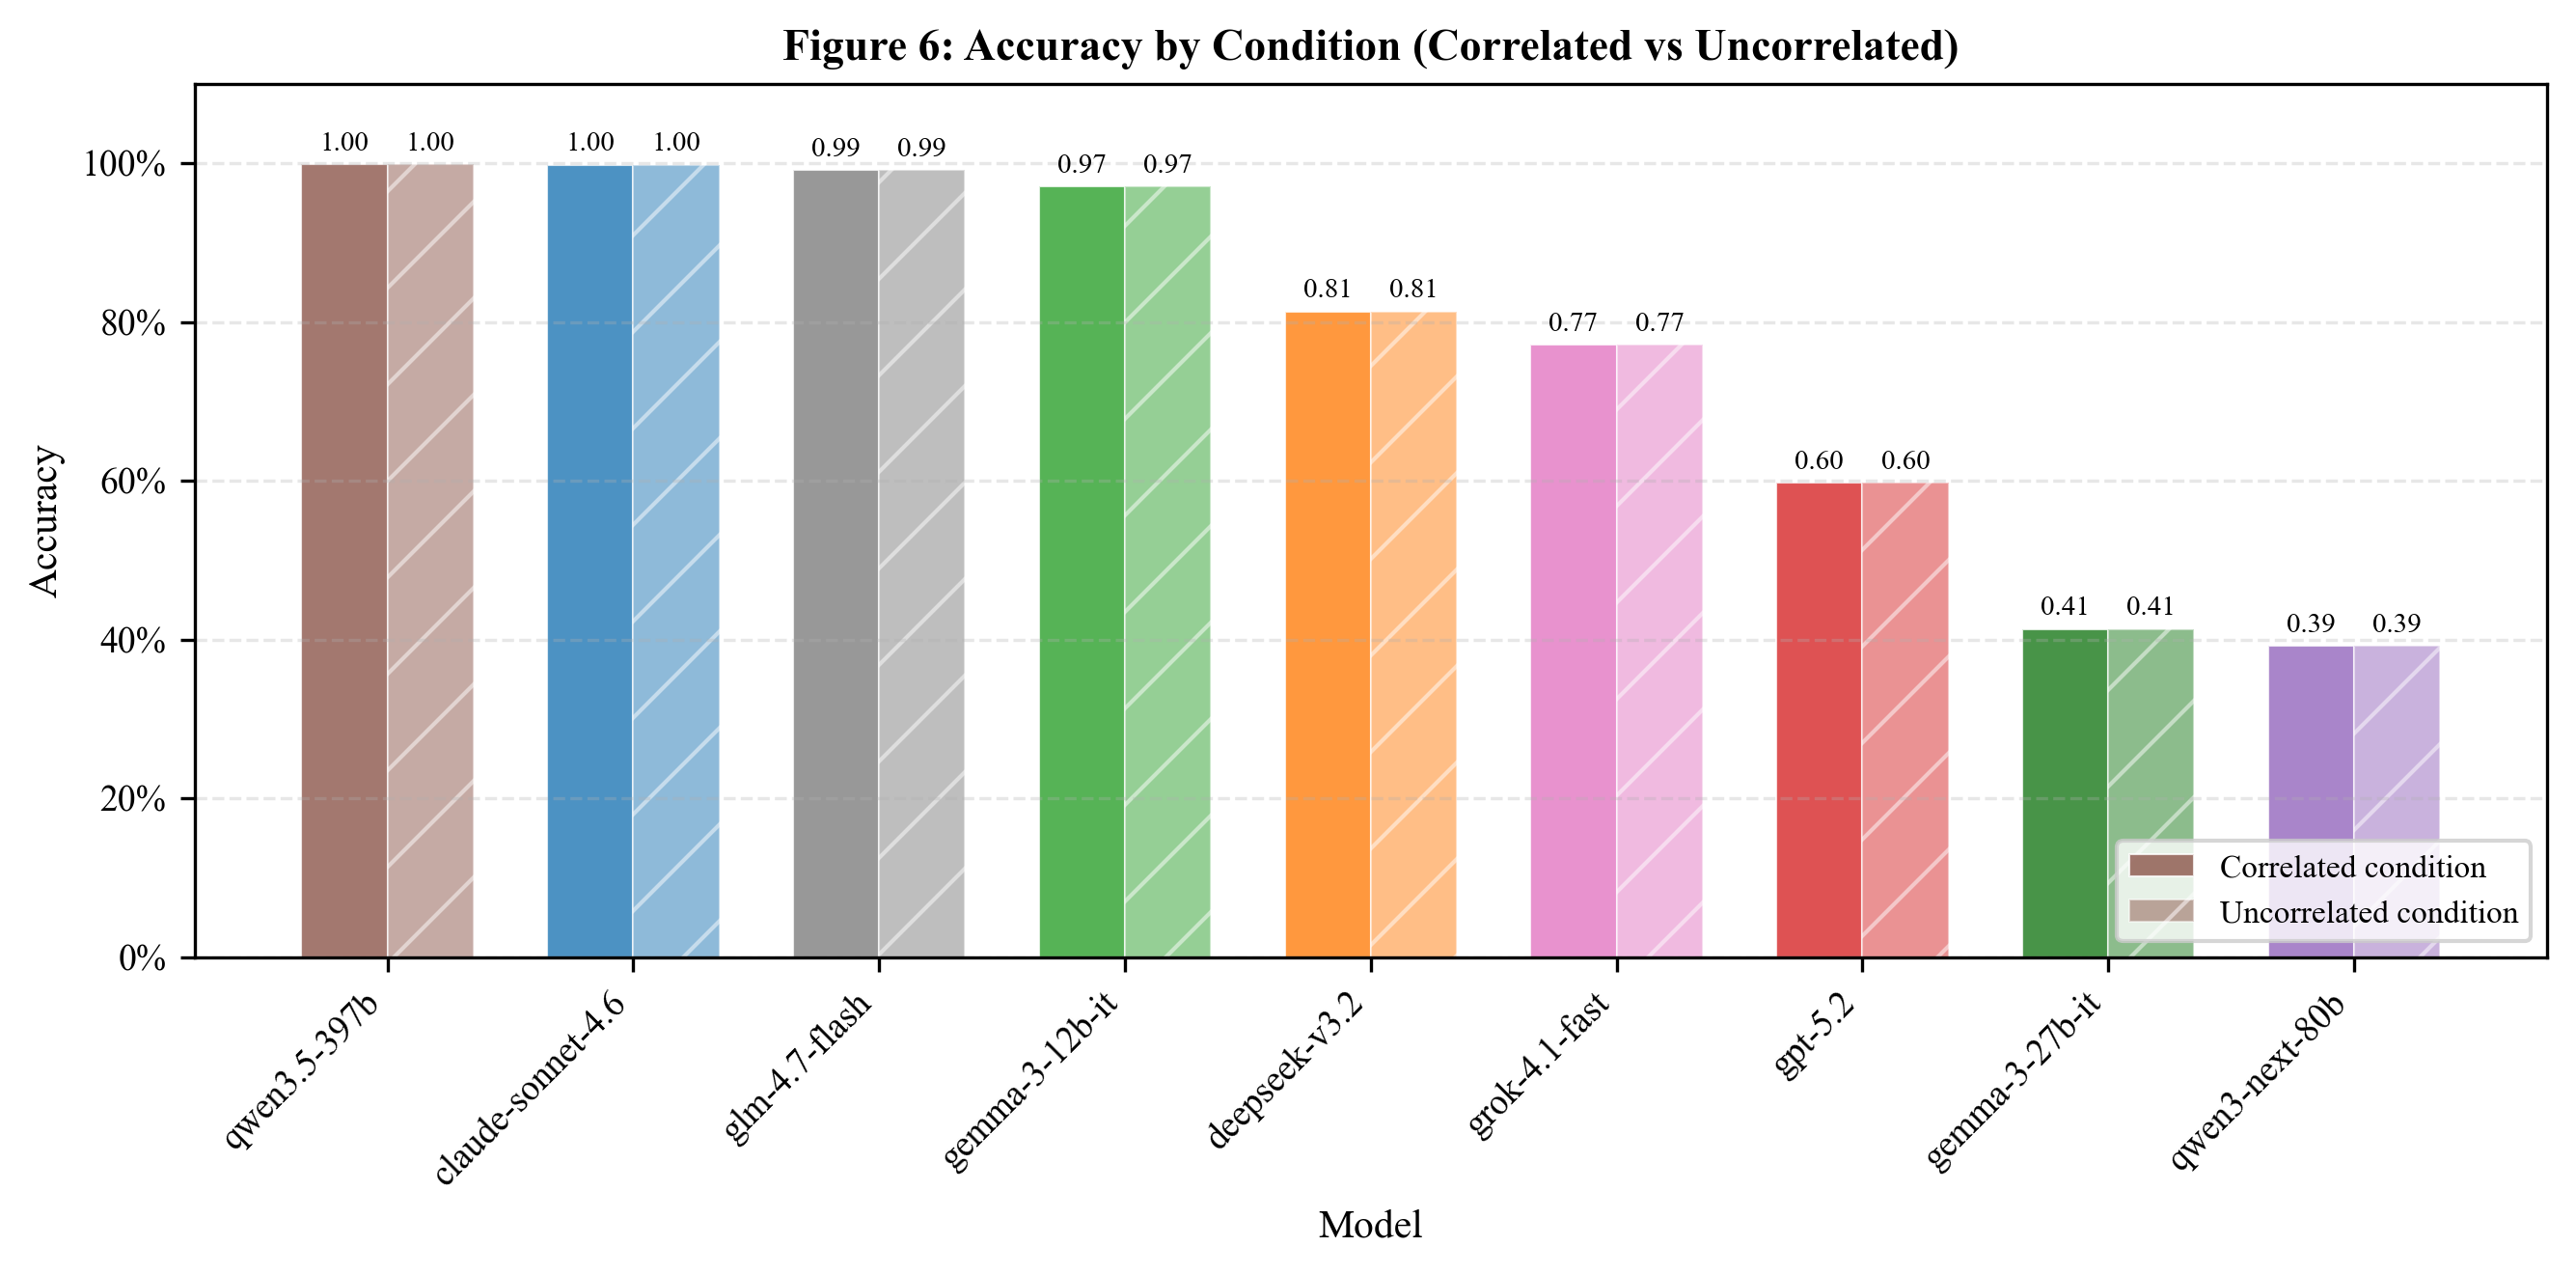
\includegraphics[width=0.48\textwidth]{../experiments_raw_results/linda-problem/figures/linda_accuracy_by_condition.png}
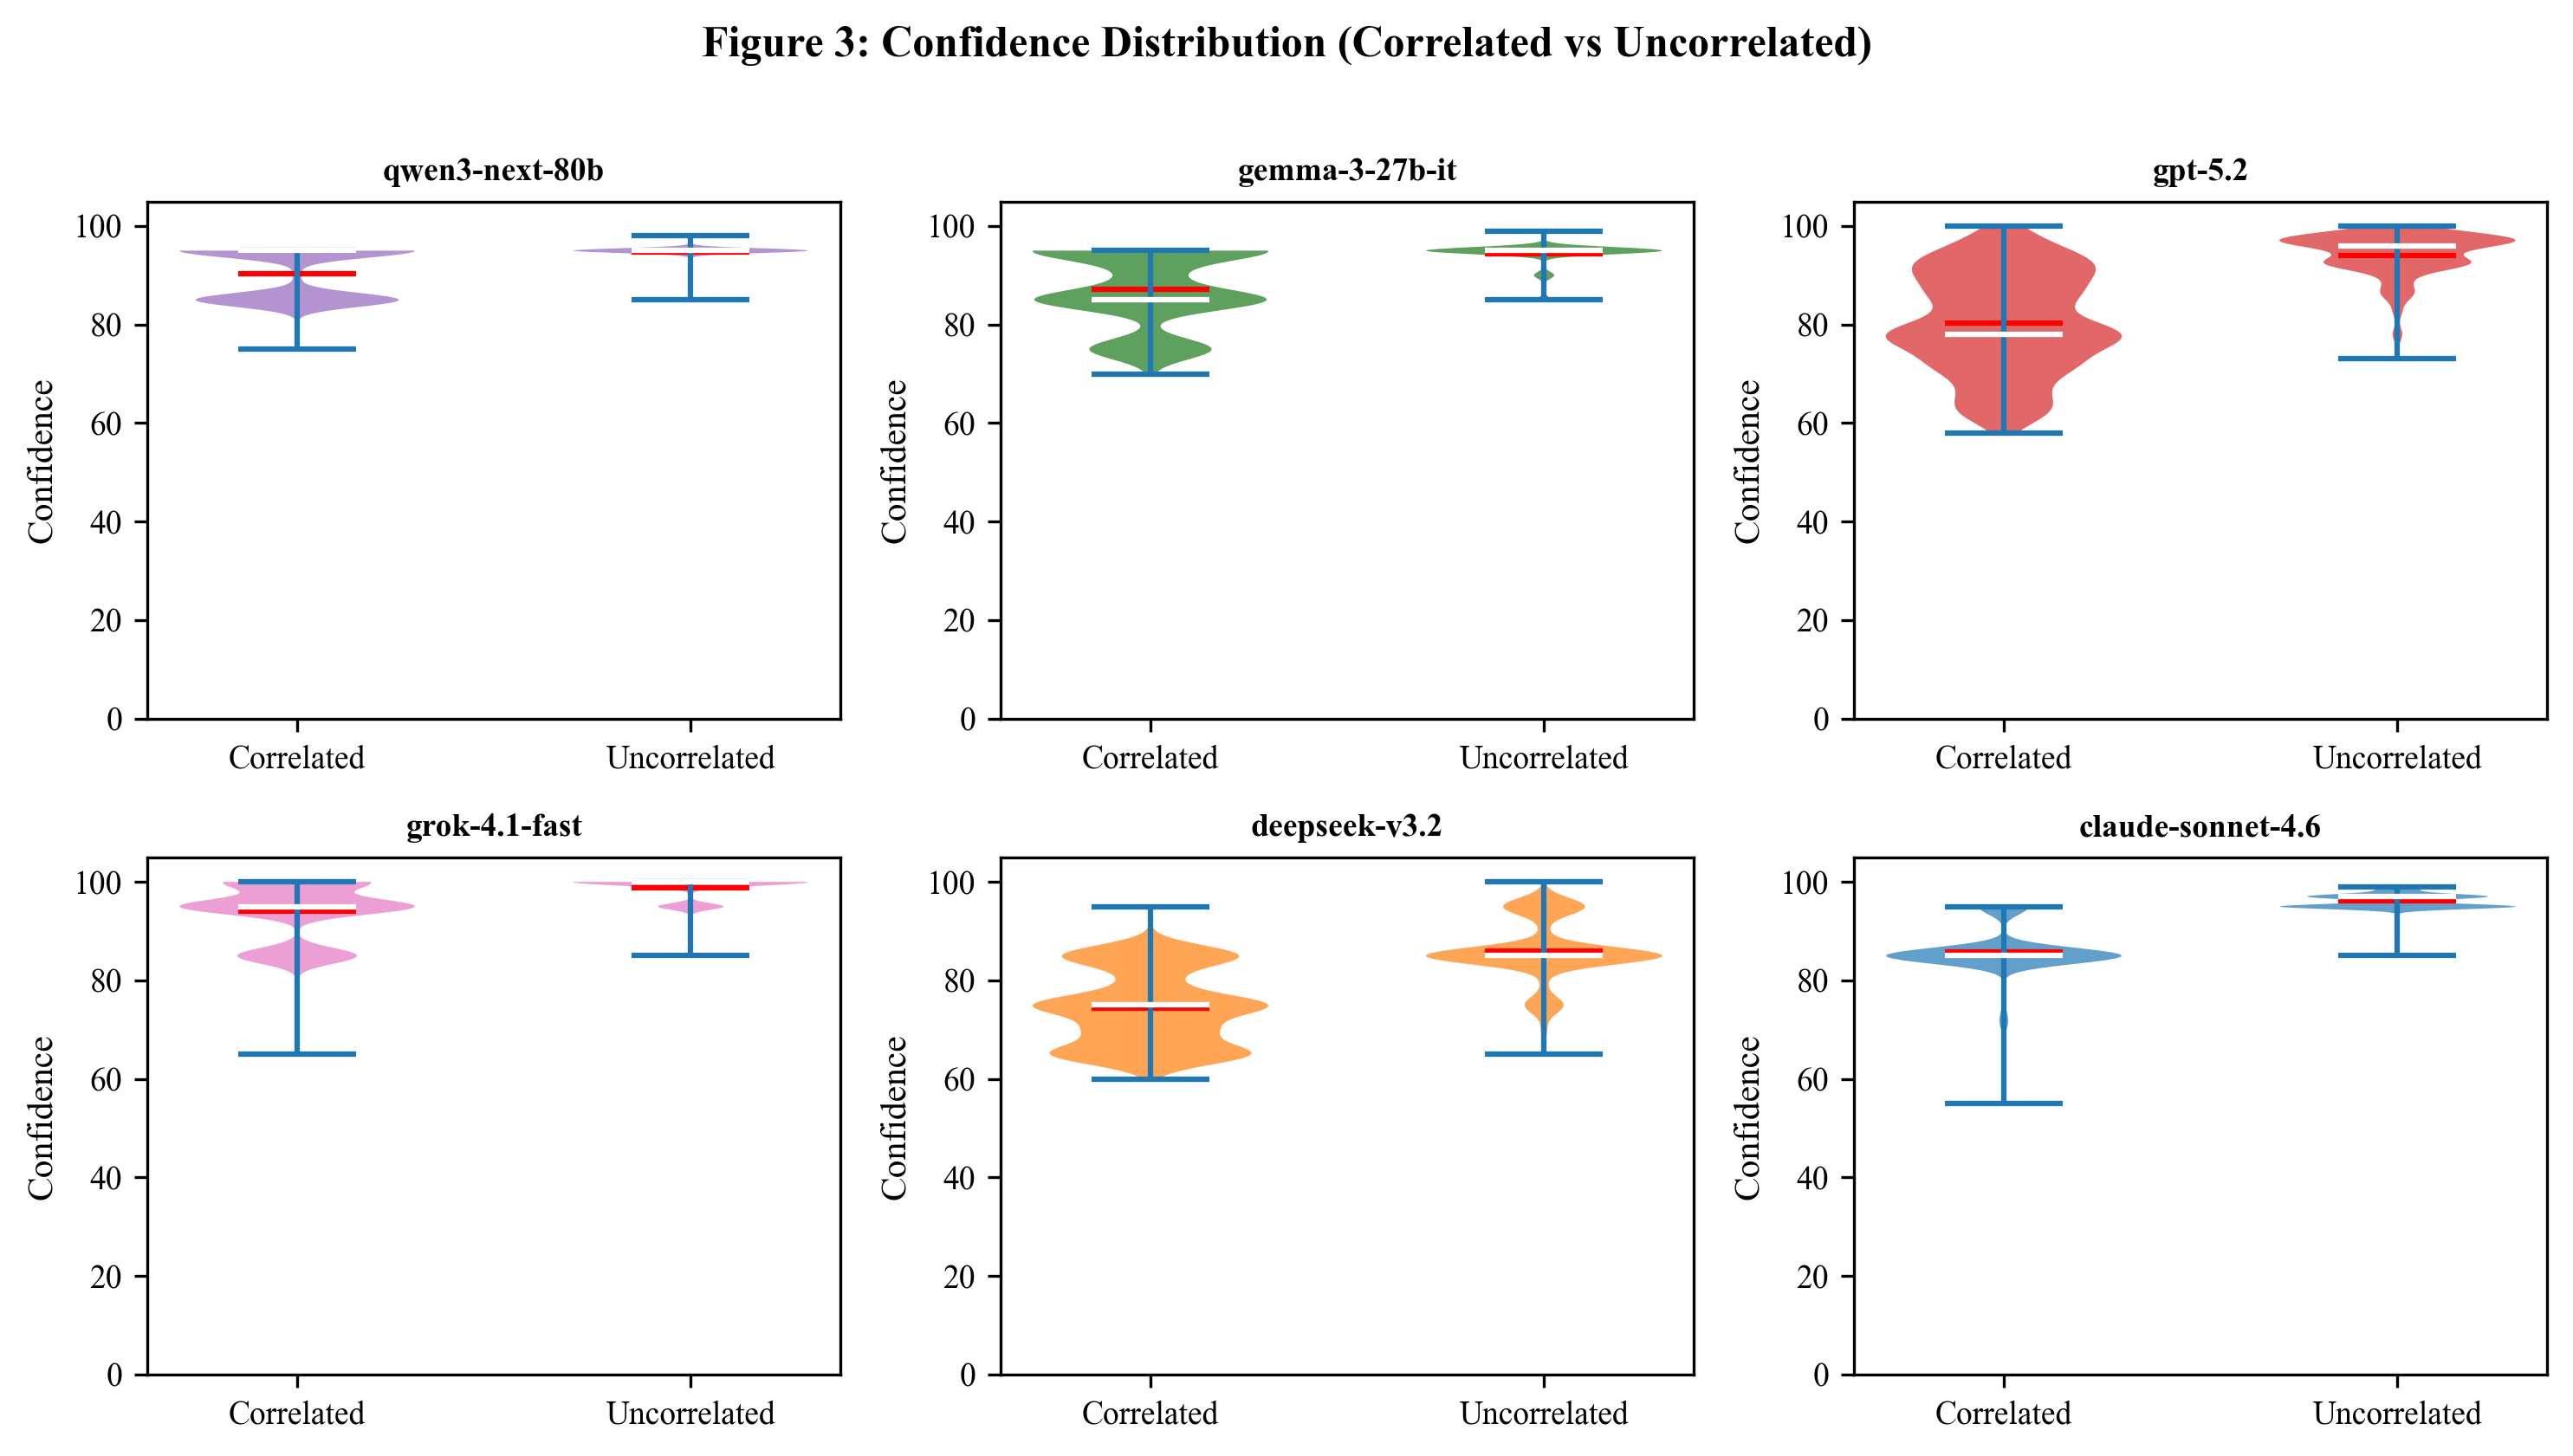
\includegraphics[width=0.48\textwidth]{../experiments_raw_results/linda-problem/figures/linda_confidence_violin.png}
\caption{Left: The dramatic performance gap between conditions. Right: Distribution of confidence, showing models are "certainly wrong" in the correlated condition.}
\end{figure}

\begin{figure}[h!]
\centering
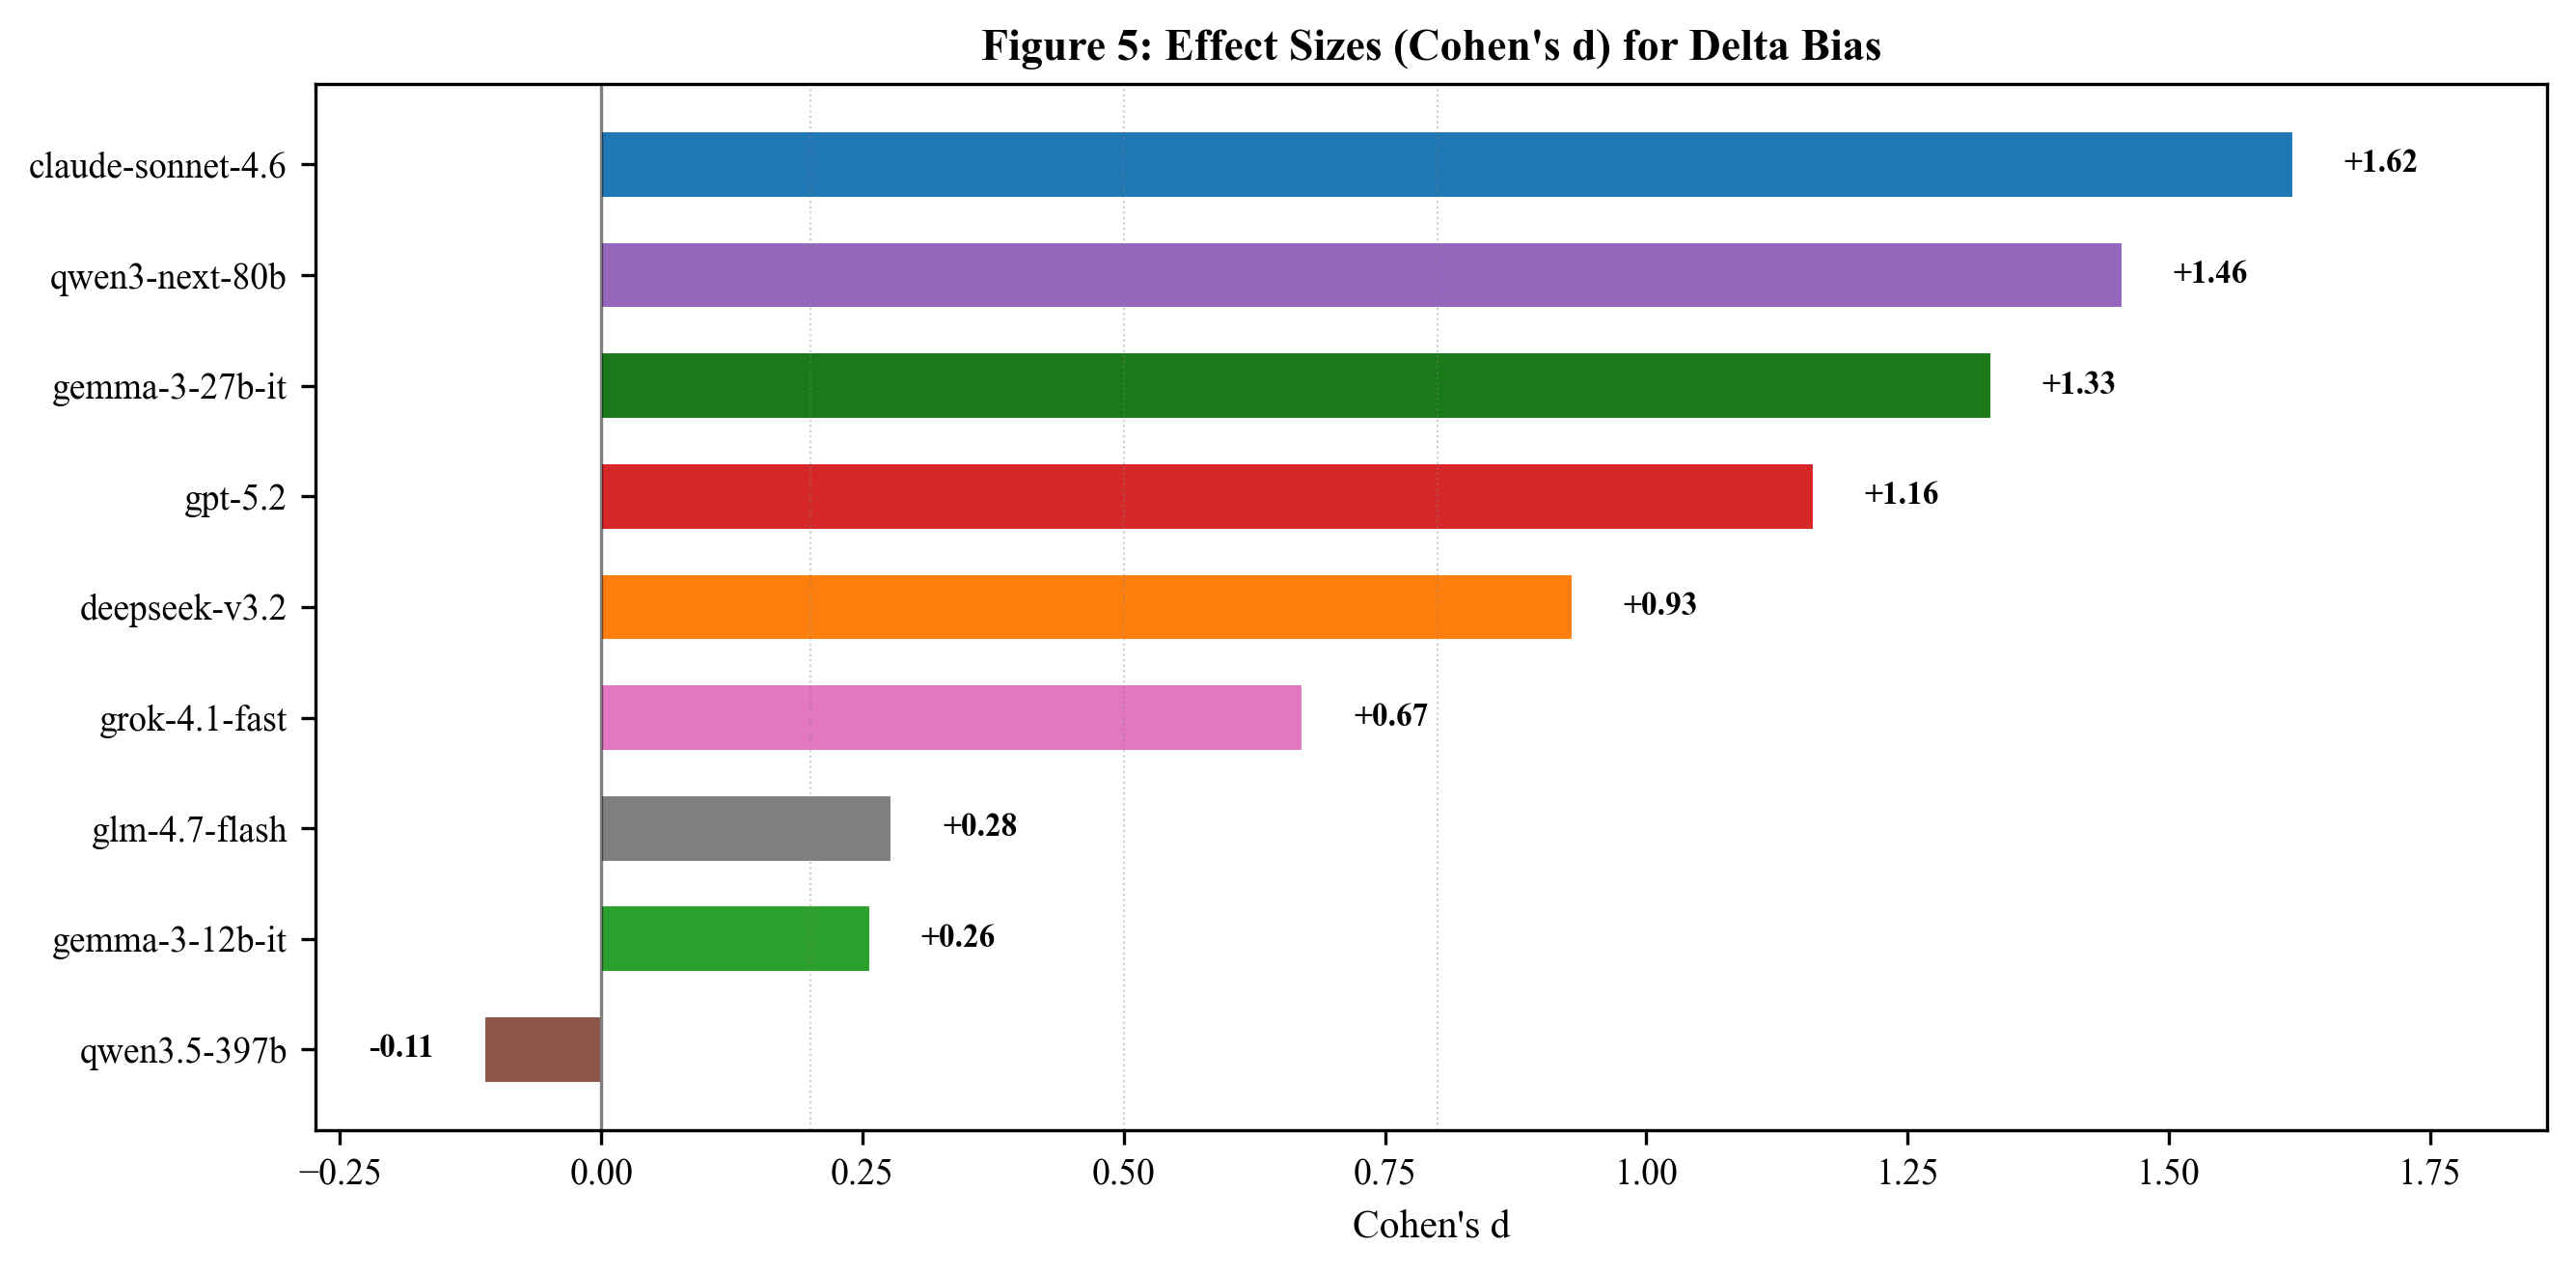
\includegraphics[width=0.48\textwidth]{../experiments_raw_results/linda-problem/figures/linda_effect_sizes_forest.png}
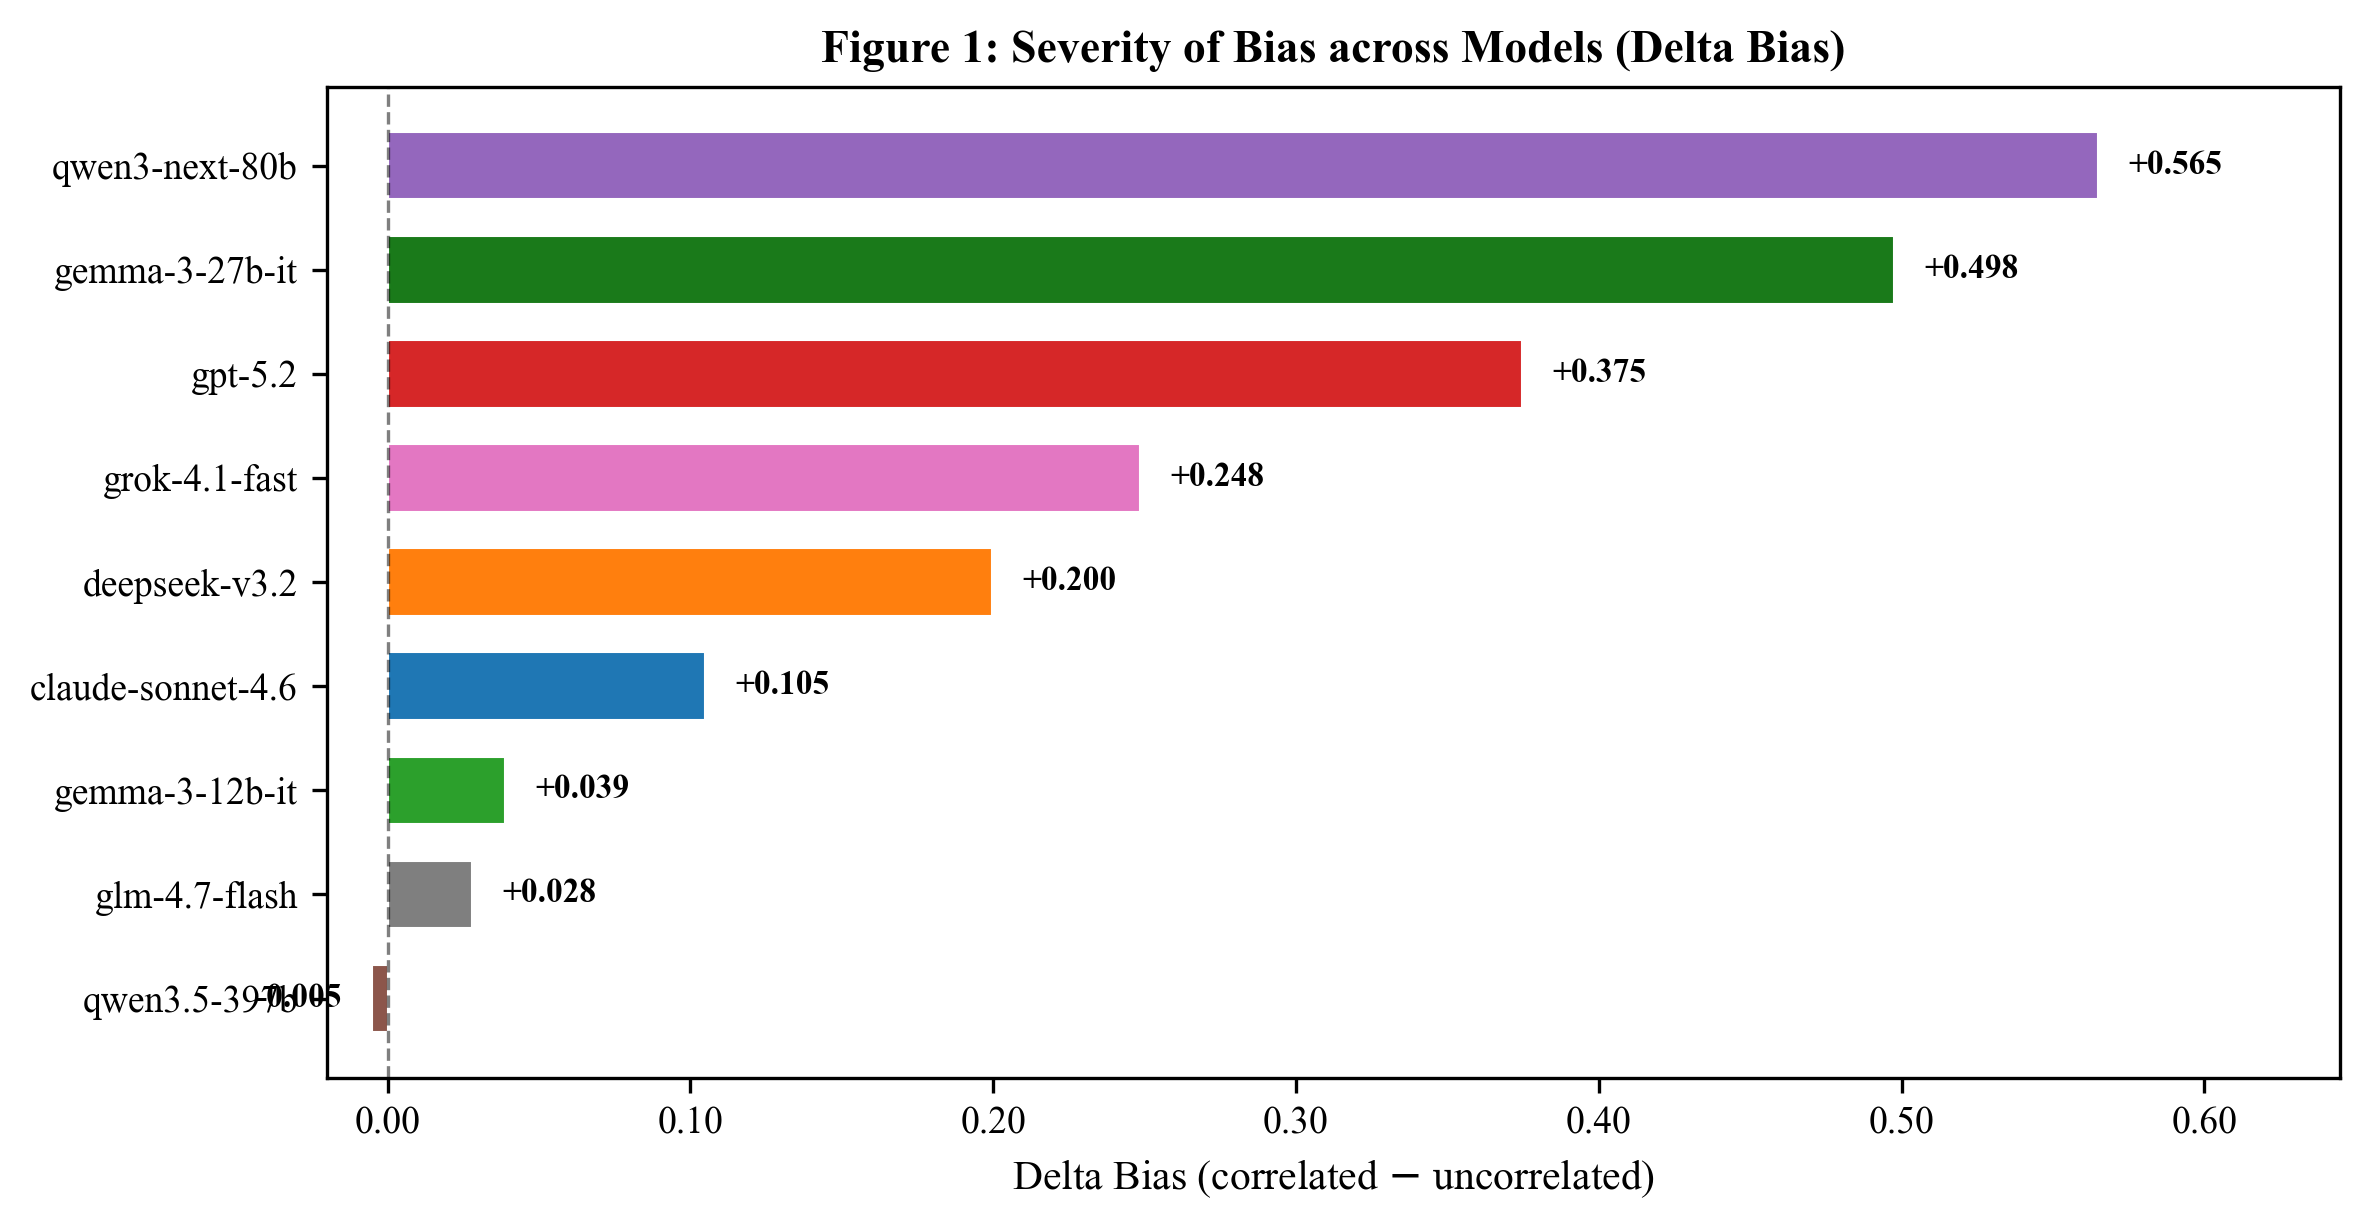
\includegraphics[width=0.48\textwidth]{../experiments_raw_results/linda-problem/figures/linda_delta_bias_bar.png}
\caption{Left: Effect sizes (Cohen's $d$). Right: The latent pressure of the bias measured through confidence shift.}
\end{figure}

\subsection*{1.7. Comparison with Human Data}
Our experimental protocol --- a binary choice between $T$ and $T \land F$ --- closely mirrors the ``transparent'' variant of Tversky and Kahneman's~\cite{tversky1983extensional} original paradigm, as well as the protocol of Charness, Karni, and Levin~\cite{charness2010social}.

\textbf{Tversky and Kahneman (1983)} tested several variants. In the most comparable ``transparent'' binary choice (only $T$ vs.\ $T \land F$), \textbf{85\%} of participants chose the conjunction as more probable. Even when an explicit hint about the logical inclusion relation was provided, the fallacy rate remained at \textbf{57\%}. In the within-subject ranking format (8 alternatives), 85--87\% ranked $T \land F$ above $T$.

\textbf{Charness, Karni, and Levin (2010)} replicated the transparent binary test with UCSB students, manipulating incentives and group discussion:

\begin{table}[h!]
\centering
\caption{Human Conjunction Fallacy Rates (Charness et al., 2010)}
\label{tab:human_linda}
\begin{tabular}{lccc}
\toprule
\textbf{Condition} & \textbf{$N$} & \textbf{Errors} & \textbf{Fallacy Rate} \\
\midrule
Individuals, no incentives       & 86  & 50  & 58.1\% \\
Individuals, \$4 incentive       & 94  & 31  & 33.0\% \\
Pairs, no incentives             & 56  & 27  & 48.2\% \\
Pairs, \$4 incentive             & 38  & 5   & 13.2\% \\
Triples, no incentives           & 39  & 10  & 25.6\% \\
Triples, \$4 incentive           & 48  & 5   & \textbf{10.4\%} \\
\bottomrule
\end{tabular}
\end{table}

Monetary incentives and group discussion substantially reduce the fallacy, but even triples with \$4 payment do not eliminate it (10.4\%).

\textbf{Hertwig and Chase (1998)} demonstrated that the \textit{response format} modulates the effect: ranking yields $\sim$78\% fallacy rate, while numerical probability estimation reduces it to $\sim$42\%. This is relevant to our setting, as models produce both a binary choice and a numerical confidence score.

\textbf{Comparison with LLMs.} The following table places our results alongside the human baselines:

\begin{table}[h!]
\centering
\caption{Conjunction Fallacy: Humans vs.\ LLMs}
\label{tab:human_vs_llm}
\begin{tabular}{lc}
\toprule
\textbf{Group / Model} & \textbf{Fallacy Rate} \\
\midrule
\multicolumn{2}{l}{\textit{Humans (binary choice, no incentives)}} \\
\quad Tversky \& Kahneman (1983)     & 85\% \\
\quad Charness et al.\ (2010)        & 58\% \\
\multicolumn{2}{l}{\textit{Humans (triples + \$4 incentive)}} \\
\quad Charness et al.\ (2010)        & 10\% \\
\midrule
\multicolumn{2}{l}{\textit{LLMs (Correlated condition, this work)}} \\
\quad qwen3-next-80b                 & 60.8\% \\
\quad gemma-3-27b-it                 & 58.7\% \\
\quad gpt-5.2                        & 40.2\% \\
\quad grok-4.1-fast                  & 22.9\% \\
\quad deepseek-v3.2                  & 18.7\% \\
\quad gemma-3-12b-it                 & 2.7\% \\
\quad glm-4.7-flash                  & 0.8\% \\
\quad claude-sonnet-4.6              & 0.2\% \\
\quad qwen3.5-397b                   & $\sim$0\% \\
\bottomrule
\end{tabular}
\end{table}

The highest-bias LLMs (\texttt{qwen3-next-80b}: 60.8\%, \texttt{gemma-3-27b-it}: 58.7\%) match the fallacy rate of unincentivized individual humans (58--85\%). The best LLMs (\texttt{qwen3.5-397b}: $\sim$0\%, \texttt{claude-sonnet-4.6}: 0.2\%) substantially outperform even incentivized human triples (10.4\%). A critical structural difference remains: in the original human studies, some participants committed the ``double fallacy'' (rating $T$ alone as more probable than $T$ in the control condition) or errors in the uncorrelated condition. In our data, $n_{22} = 0$ and $n_{12} = 0$ for all nine models --- no model ever failed the control task. LLM errors are \textit{purely} driven by semantic correlation, making the bias more structured than in humans.
